\chapter{Comparación con el FHCP Challenge}
\label{cap:bench}

\section{El FHCP Challenge}
El FHCP Challenge Set fue publicado por el Flinders Hamiltonian Cycle Project, de la Universidad
Flinders en Australia \cite{aco8,aco9}. Tiene 1\,001 grafos de entre 66 y 9\,528 vértices (en
promedio, poco más de 3\,000), y de todos se sabe que tienen ciclo hamiltoniano.

Con este conjunto se organizó un concurso del 30 de septiembre de 2015 al 30 de septiembre de
2016. Las reglas, según la página oficial \cite{aco9}, eran:
\begin{itemize}
  \item Las soluciones se entregaban en el formato TOUR, el mismo que usamos nosotros.
  \item Una solución contaba solo si era un ciclo hamiltoniano válido.
  \item Ganaba quien resolviera los 1\,001 grafos o, si nadie lo lograba, quien resolviera más.
        En caso de empate, ganaba quien hubiera entregado primero.
  \item El premio era de 1\,001 dólares.
\end{itemize}

Nadie resolvió los 1\,001 grafos. Los ganadores fueron Nathann Cohen y David Coudert, que
encontraron ciclos hamiltonianos en \textbf{985 grafos} \cite{aco9}.

Para nuestro trabajo tomamos el mismo criterio de éxito (un ciclo verificado) y el mismo formato
de salida. La diferencia es que nosotros comparamos con las \emph{soluciones oficiales} que publica
el proyecto, una para cada grafo.

\section{Calidad de las soluciones}
En este problema, una solución es correcta o no lo es: no hay ciclos hamiltonianos ``mejores''
que otros. Todas las soluciones que encontraron nuestros algoritmos las guardamos en formato TOUR
y pasaron el mismo verificador que acepta las soluciones oficiales
(sección~\ref{sec:verificacion}). Así que, en los grafos que resolvimos, nuestra solución es tan
válida como la oficial. En los que no resolvimos, lo que podemos reportar es cuántas aristas
faltaron.

\section{Grafos resueltos (experimento B)}
En el experimento B corrimos \alg{ABC} y \alg{ACO + Pósa} sobre los primeros 100 grafos del
conjunto, con 2 semillas y 2 minutos por corrida (tabla~\ref{tab:benchmarking}).

\begin{table}[H]
\centering\small\filas
\caption{Experimento B: grafos resueltos en al menos una de las \semillasB{} semillas, comparados con las soluciones oficiales.}
\label{tab:benchmarking}
\resizebox{\textwidth}{!}{% Generado por Reporte/actualizar.py; no editar a mano.
\begin{tabular}{lrrrrr}
\toprule
Instancias & $n$ & ACO + Pósa & ABC & Cualquiera de los dos & Con solución oficial \\
\midrule
graph1--graph25 & 66--204 & 9 & 8 & 9 & 25 \\
graph26--graph50 & 210--348 & 0 & 6 & 6 & 25 \\
graph51--graph75 & 354--468 & 0 & 2 & 2 & 25 \\
graph76--graph100 & 471--558 & 0 & 3 & 3 & 25 \\
\midrule
Total & & 9 & 19 & 20 & 100 \\
\bottomrule
\end{tabular}
}
\end{table}

\alg{ABC} resolvió \resueltasBABC{} de los \grafosB{} grafos y \alg{ACO + Pósa},
\resueltasBACOposa{}. Juntos resolvieron 20, porque 8 de los 9 grafos que resolvió
\alg{ACO + Pósa} también los resolvió \alg{ABC} (la excepción es graph1). La diferencia más importante es el tamaño:
\alg{ACO + Pósa} no resolvió ningún grafo después de graph25 (más de 204 vértices), mientras que
\alg{ABC} siguió resolviendo algunos hasta los 558 vértices.

\begin{table}[H]
\centering\filas
\caption{Experimento B: resumen por algoritmo.}
\label{tab:resumenB}
\resizebox{\textwidth}{!}{% Generado por Reporte/actualizar.py; no editar a mano.
\begin{tabular}{lrcrrrrr}
\toprule
Algoritmo & Éxitos & Tasa de éxito [IC 95\,\%] & Grafos resueltos & Tiempo (s) & Evaluaciones hasta el éxito & Aristas faltantes (prom.) & F1 \\
\midrule
ACO + Pósa & 14/200 & 0.07 [0.04, 0.11] & 9/100 & 112.5 $\pm$ 28.7 & 1\,281 & 30.54 & 0.13 \\
ABC & 30/200 & 0.15 [0.11, 0.21] & 19/100 & 105.7 $\pm$ 35.9 & 291\,682 & 2.50 & 0.26 \\
\bottomrule
\end{tabular}
}
\end{table}

\begin{figure}[H]
\centering
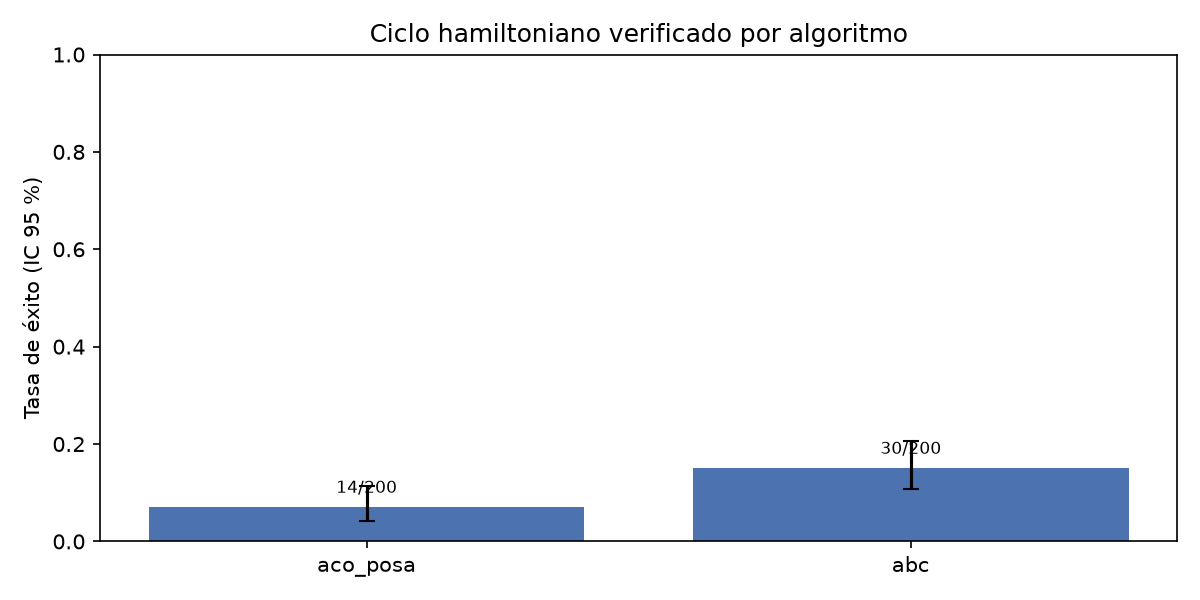
\includegraphics[width=.7\textwidth]{disenoB/exito_algoritmos.png}
\caption{Experimento B: tasa de éxito por algoritmo.}
\label{fig:exitoB}
\end{figure}

Los grafos que resolvió cada algoritmo fueron:
% Generado por Reporte/actualizar.py; no editar a mano.
\begin{description}
\item[ACO + Pósa] graph1, graph2, graph4, graph6, graph8, graph10, graph14, graph18, graph23.
\item[ABC] graph2, graph4, graph6, graph8, graph10, graph14, graph18, graph23, graph27, graph31, graph35, graph39, graph43, graph47, graph52, graph67, graph78, graph85, graph99.
\end{description}


\begin{figure}[H]
\centering
\begin{subfigure}{.49\textwidth}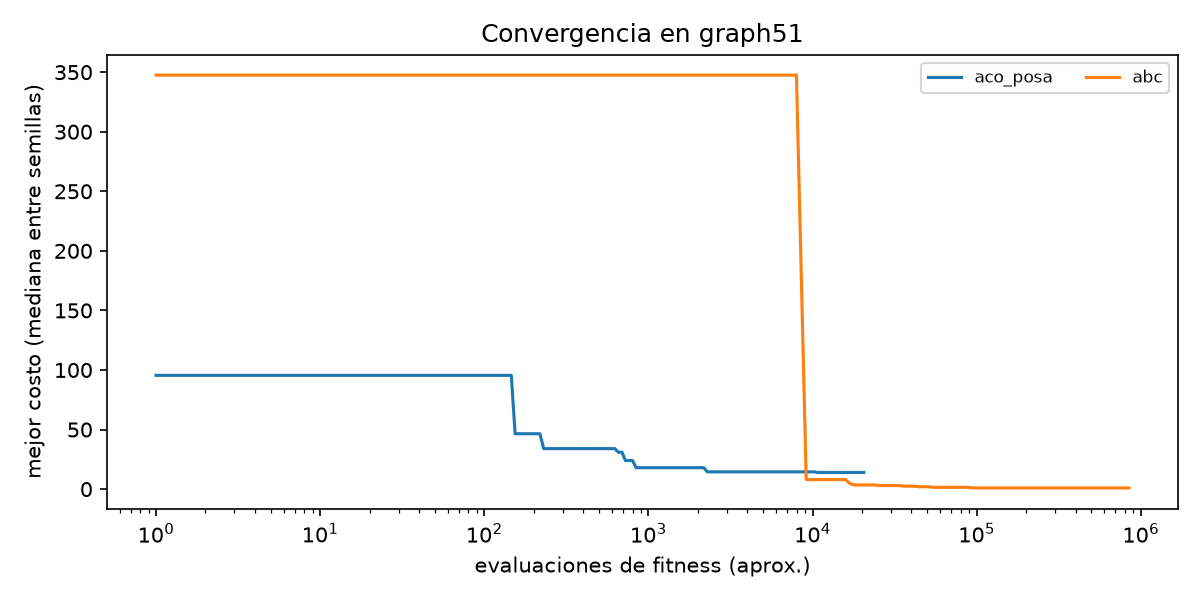
\includegraphics[width=\textwidth]{disenoB/convergencia_graph51.png}\caption{graph51}\end{subfigure}
\begin{subfigure}{.49\textwidth}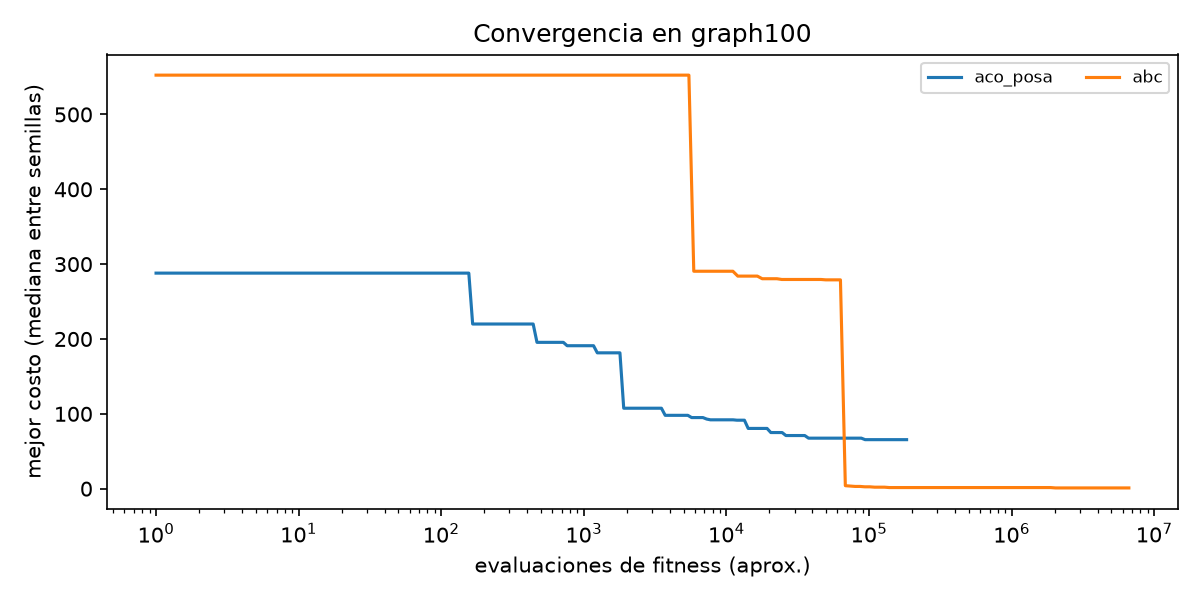
\includegraphics[width=\textwidth]{disenoB/convergencia_graph100.png}\caption{graph100}\end{subfigure}
\caption{Experimento B: convergencia en dos grafos medianos.}
\label{fig:convB}
\end{figure}

\section{Nuestros resultados frente a los mejores}
La diferencia con los mejores resultados es grande. Los ganadores del concurso resolvieron 985 de
los 1\,001 grafos, incluidos los más grandes. Nosotros, en los 100 grafos más pequeños, resolvimos
20 en total. Creemos que esta diferencia se explica por tres razones:
\begin{enumerate}
  \item \textbf{Algoritmos especializados.} Los mejores métodos para este problema están
        diseñados específicamente para ciclos hamiltonianos o para el TSP. Un ejemplo es la
        heurística \emph{Snakes and Ladders}, desarrollada por el mismo grupo de investigación del
        FHCP \cite{slh2014}. Otro es convertir el problema en un TSP y resolverlo con programas como
        LKH \cite{lkh2000}, que tienen búsquedas locales muy potentes. Nuestras metaheurísticas son
        de uso general.
  \item \textbf{Tiempo de cómputo.} Nosotros dimos 2 minutos por corrida. Un concurso de un año
        permite usar horas o días por grafo.
  \item \textbf{Implementación.} Nuestro código está en Python puro, que es bastante más lento que
        el C o C++ que suelen usar estas herramientas.
\end{enumerate}

Aun así, nuestros resultados dejan una lección clara: los dos algoritmos que mejor funcionaron
son los que buscan aprovechando la estructura del grafo (aristas reales, reparaciones locales y
rotaciones), que es también la idea en la que se basan los métodos especializados.
